\chapter{Конструкторский раздел}

В данным разделе представлены требования к разрабатываемому методу и программному комплексу, которые реализуют интерфейс для этого метода. Будет рассмотрена архитектура метода, определяющая его структуру и компоненты, а также будет приведено описание структуры программного комплекса, который обеспечивает реализацию данного метода и предоставляет пользовательский интерфейс для его использования.

\section{Требования к разрабатываемому методу}

Метод фильтрации малоразмерных шумов на цветных изображениях должен:
\begin{itemize}
    \item обрабатывать входные изображения в трех форматах данных: PNG, JPG, JPEG, а также гарантируется, что цветное изображение использует трехканальную схему хранения;
    \item обрабатывать входные изображения в произвольном разрешении;
    \item производить очистку входного цветного изображения от малоразмерных помех.
\end{itemize}

\section{Требования к разрабатываемому программному комплексу}
Программный комплекс, который реализует интерфейс для разработанного метода обязан:
\begin{itemize}
    \item предоставлять функцию загрузки изображений из произвольной директории;
    \item предоставлять функцию сохранения результатов работы программы в пути, указанном пользователем;
    \item предоставлять функцию подсчета метрик оценки качества восстановленного изображения.
\end{itemize}

\section{Проектирование метода устранения помех}

Задачу устранения помех можно подразбить на две подзадачи:
\begin{itemize}
    \item выявление шумов на изображении;
    \item удаление шумов с изображения.
\end{itemize}

Для решения поставленной задачи будет использоваться модель сверточной нейронной сети, обрабатывающая цветные изображения размерностью 32x32 пикселей и состоящая из двух подсетей на каждую из подзадач. Тогда для обработки изображений произвольной размерности необходимо предварительно разбить его на составляющие патчи размерностью 32х32, выполнить их фильтрацию по отдельности и объединить обратно.

В качестве основы была выбрана архитектура UNet, модифицированная путем добавления нескольких слоев предобработки изображения для формирования карт признаков шумов изображения и использования полносвязной нейронной сети в конце. Для всех сверточных слоев используется функция активации ReLu и сверточное ядро размером 3x3. Для обучения нейронной сети предполагается использовать метод обратного распространения ошибки и метод среднеквадратичного отклонения в качестве функции потерь.

Таким образом, принцип работы проектируемого метода представлен в виде IDEF0--диаграммы на рисунке \ref{fig:concept}.

\begin{figure}[h!btp]
	\centering
	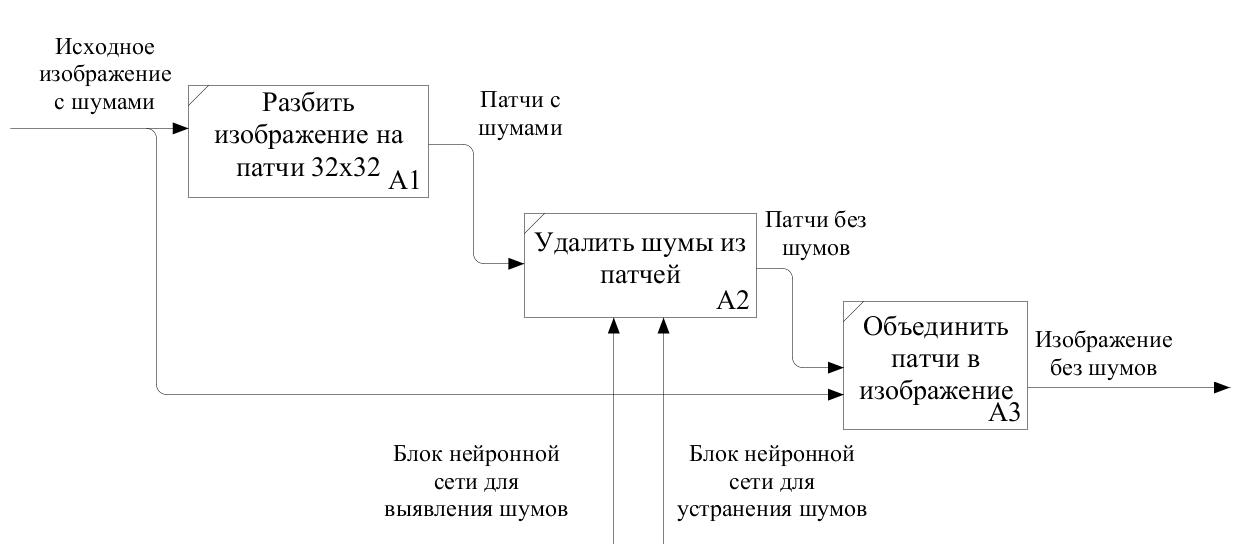
\includegraphics[scale = 0.50]{inc/analysis/02_A0.png}
	\caption{IDEF0--диаграмма первого уровня}
	\label{fig:concept}	
\end{figure}

\subsection{Подсеть для выявления помех}
На рисунке \ref{fig:my_fcn} приводится схема модели нейронной сети для выявления помех. Данная подсеть состоит из 5 сверточных слоев 3 видов:
\begin{itemize}
    \item сверточный слой 1--го типа имеет 3 входных канала, поскольку производится работа с цветными изображениями, и формирует 32 выходных канала, при этом используя ядра свертки 3х3;
    \item сверточный слой 2--го типа имеет 32 входных канала и формирует 32 выходных канала, при этом используя ядра свертки 3х3;
    \item сверточный слой 3--го типа имеет 32 входных канала и формирует 3 выходных канала с картами признаков шумов исходного изображения, при этом используя ядра свертки 3х3.
\end{itemize}

\begin{figure}[h!btp]
	\centering
	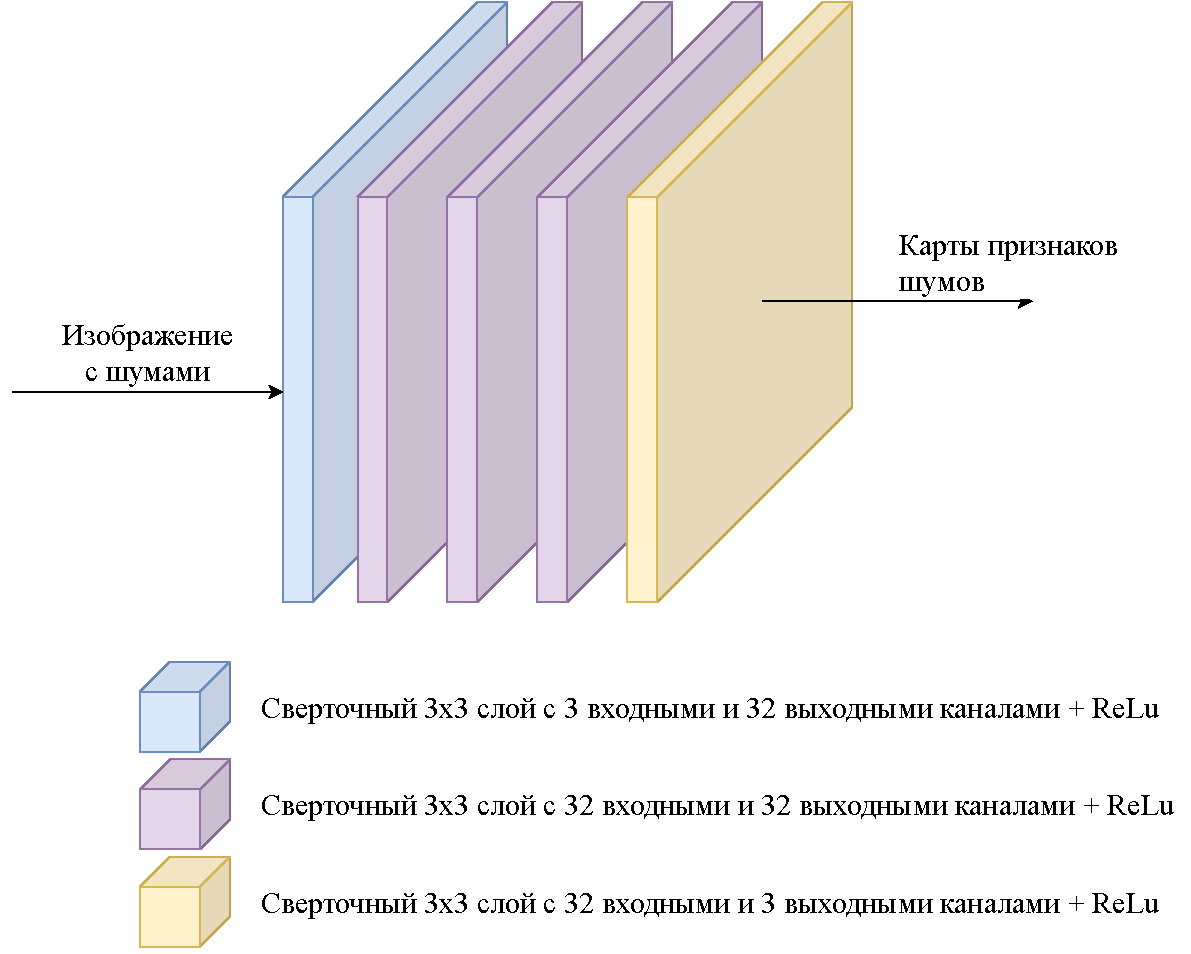
\includegraphics[scale = 0.8]{inc/design/fcn.pdf}
	\caption{Модель нейронной сети для выявления помех}
	\label{fig:my_fcn}	
\end{figure}

\subsection{Подсеть для устранения помех}
На рисунке \ref{fig:my_unet} приводится схема нейронной сети для устранения помех. Данная подсеть состоит 16 сверточных слоев 7 видов:
\begin{itemize}
    \item сверточный слой 1--го типа принимает 6 входных каналов и формирует 64 выходных каналов, при этом используя ядра свертки 3х3; 
    \item сверточный слой 2--го типа принимает 64 входных канала и формирует 64 выходных каналов, при этом используя ядра свертки 3х3; 
    \item сверточный слой 3--го типа принимает 64 входных канала и формирует 128 выходных каналов, при этом используя ядра свертки 3х3; 
    \item сверточный слой 4--го типа принимает 128 входных каналов и формирует 128 выходных каналов, при этом используя ядра свертки 3х3; 
    \item сверточный слой 5--го типа принимает 128 входных каналов и формирует 256 выходных каналов, при этом используя ядра свертки 3х3; 
    \item сверточный слой 6--го типа принимает 256 входных каналов и формирует 256 выходных каналов, при этом используя ядра свертки 3х3; 
    \item сверточный слой 7--го типа принимает 64 входных канала и формирует 3 выходных канала, при этом используя ядра свертки 3х3. 
\end{itemize}

Завершающим этапом является трехслойная полносвязная нейронная сеть со слоями размерностью 32x32x3, которые формируют итоговое изображение.

\begin{figure}[h!btp]
	\centering
	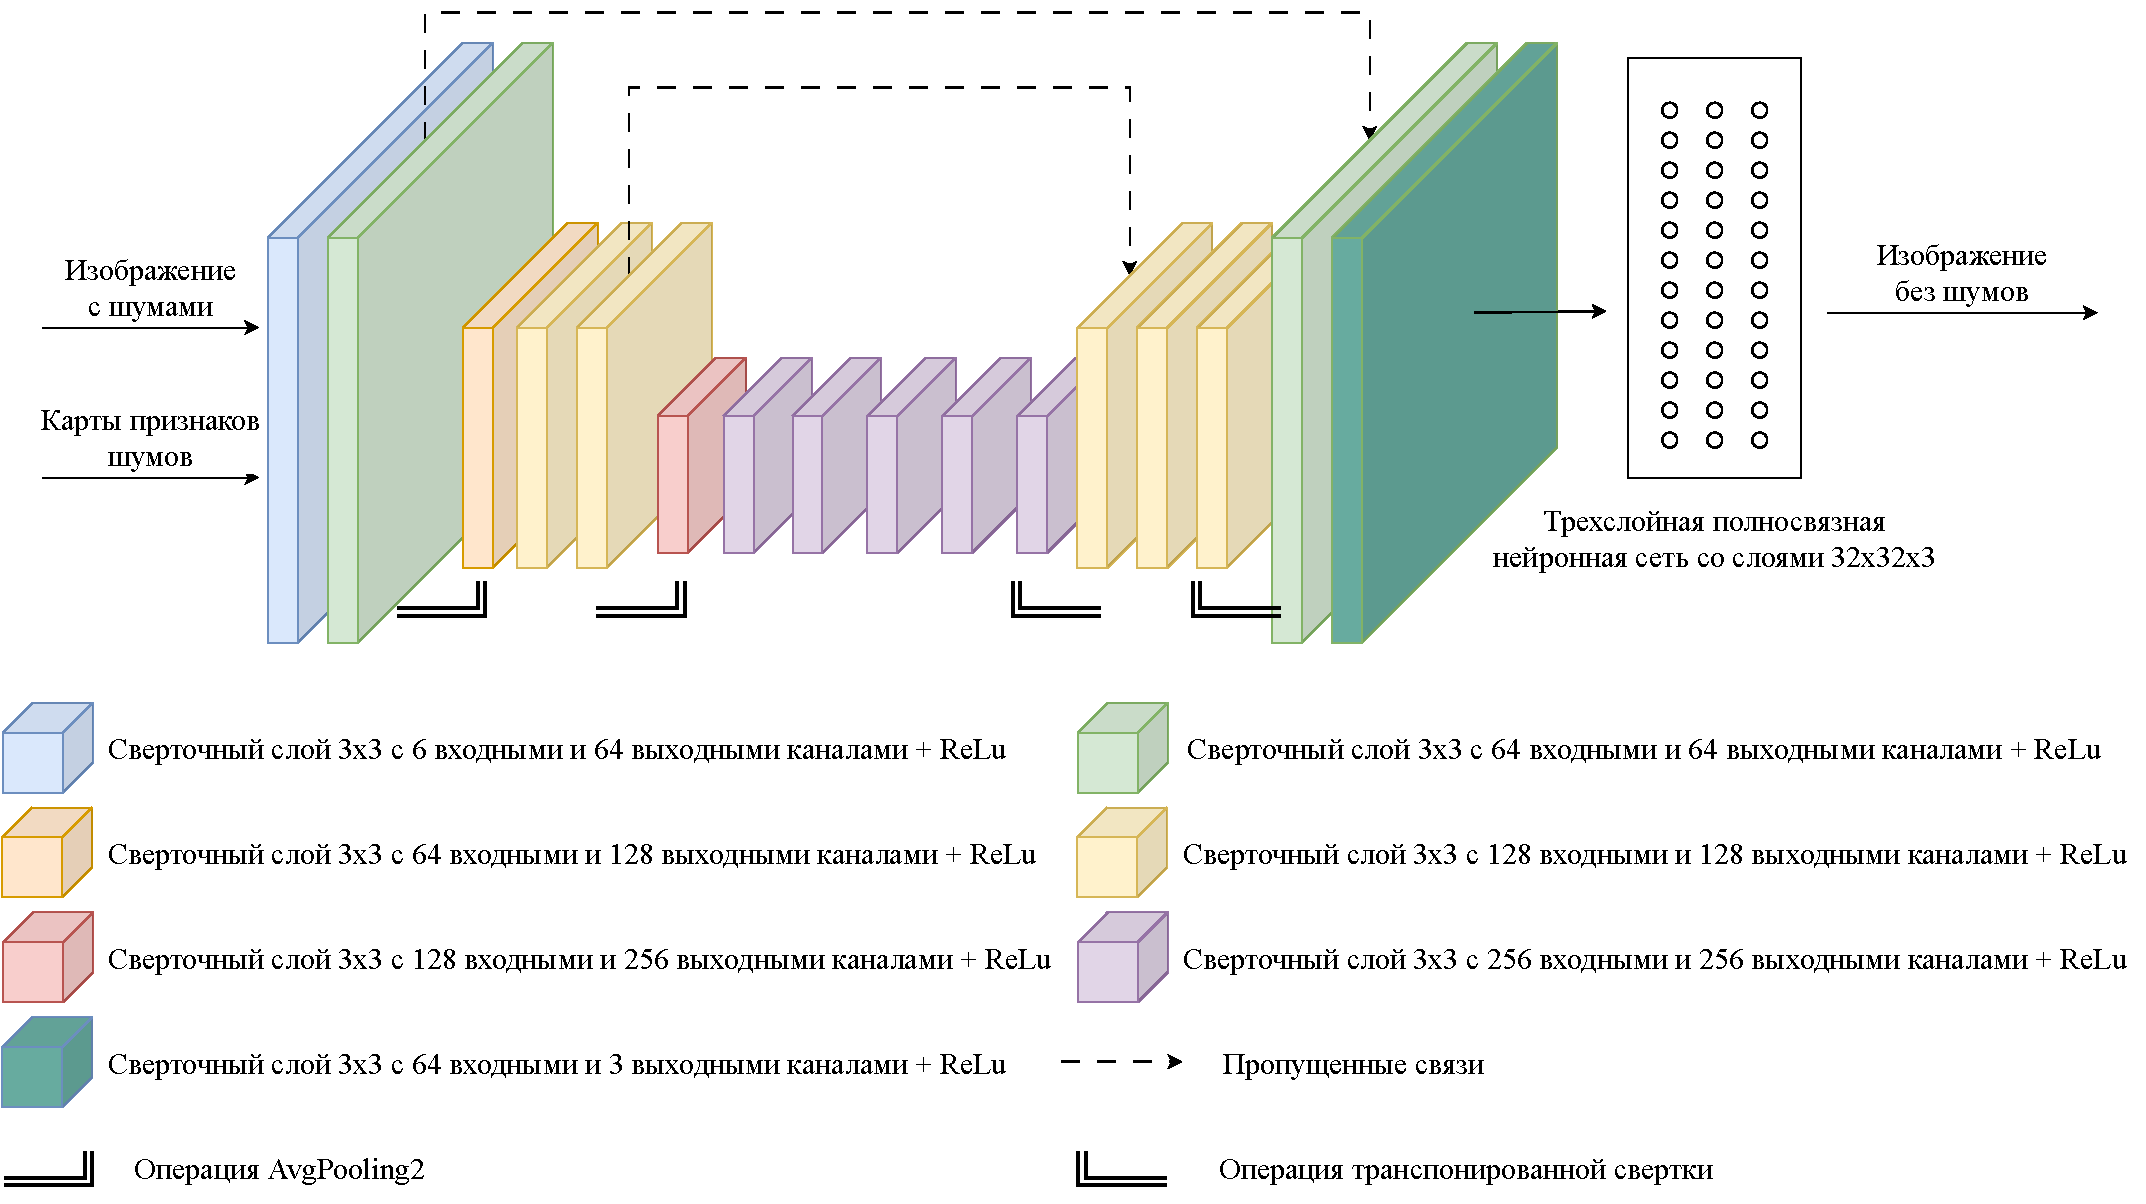
\includegraphics[scale = 0.45]{inc/design/unet.pdf}
	\caption{Модель нейронной сети для устранения помех}
	\label{fig:my_unet}	
\end{figure}

\section{Данные для обучения модели}

Современные смартфоны являются одним из самых распросраненных устройств для создания фотоснимков, однако их изображения, как правило, ухудшаются из-за повышенного уровня шума, вызванного меньшими датчиками и объективами, установленными в камерах. Ввиду описанного выше был выбран набор данных SIDD--Medium \cite{sidd} (от англ. Smartphone Image Denoising Dataset), содержащий 320 изображений, полученных с помощью следующего списка устройств: Google Pixel, iPhone 7, Samsung Galaxy S6 Edge, Motorola Nexus 6, LG G4.

Сцены запечатлены в различных условиях: в условии низкой освещенности, в условии нормальной яркости, а также в условии высокой экспозиции. Все изображения сохранены в высоком разрешении и формате без сжатия.  

На рисунках \ref{fig:dataset_original}--\ref{fig:dataset_noisy} приведены примеры изображений из выбранного набора данных.

\begin{figure}[h!btp]
	\centering
	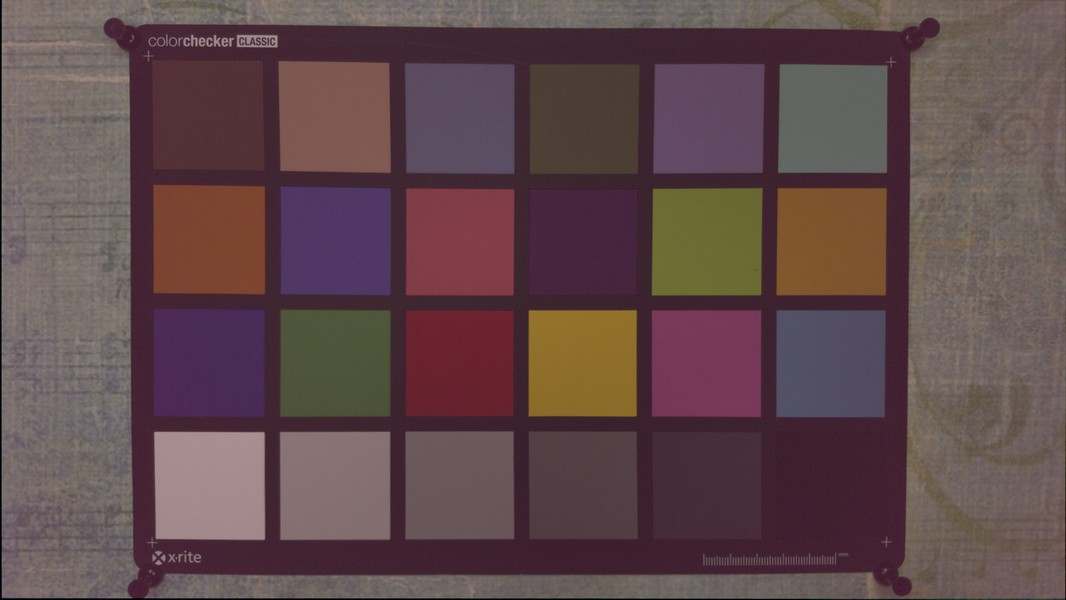
\includegraphics[scale = 0.55]{inc/design/dataset/original.jpg}
	\caption{Изображение без шумов}
	\label{fig:dataset_original}	
\end{figure}

\begin{figure}[h!btp]
	\centering
	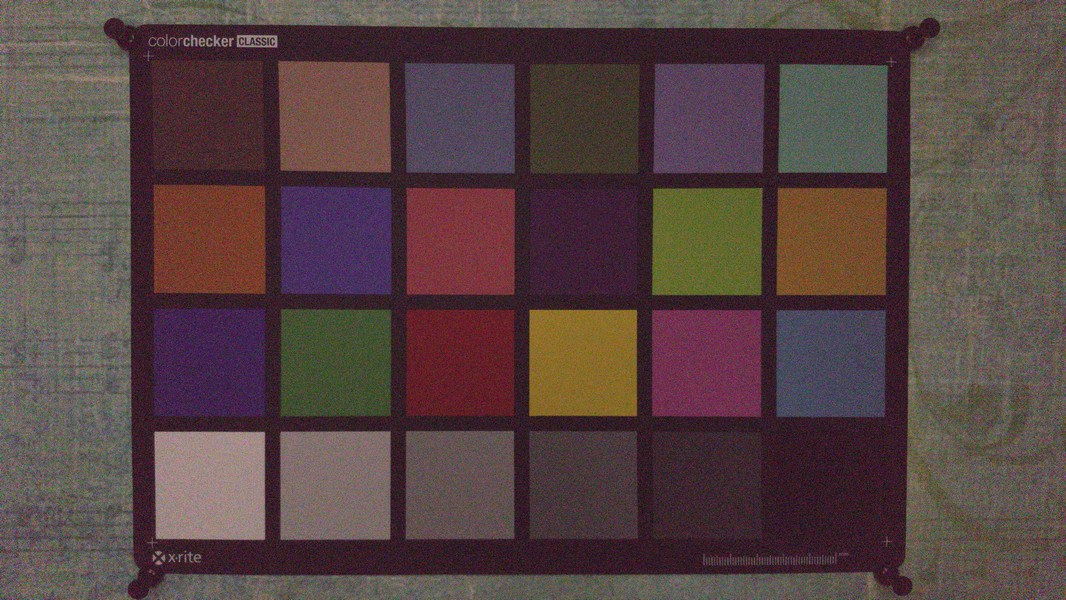
\includegraphics[scale = 0.55]{inc/design/dataset/noisy.jpg}
	\caption{Изображение с шумами}
	\label{fig:dataset_noisy}	
\end{figure}

\section{Выводы}

В данном разделе были представлены требования к разрабатываемому методу и программному комплексу, был спроектирован и описан метод фильтрации малоразмерных шумов на цветных изображениях с помощью сверточных нейронных сетей, приведены соответствующие схемы и IDEF0--диаграммы, также выполнено описание выбранного набора данных для дальнейшего обучения разработанной модели нейронной сети. 